\chapter{Auswertung der Messdaten und Diskussion}

\section{Photolumineszenz (PL) und Direktionalität}~\label{sec:PL_u_Direktionalitaet}
Die gemessene Photolumineszenz der Probe(\ref{fig:probe})
ist in Abbildung~\ref{fig:photo} zu sehen. Die Probentemperatur hat $T = \SI{4}{\kelvin}$ betragen.
Das Maximum der PL liegt bei $\SI{738}{\nano\meter}$ (vgl. Abbildung~\ref{fig:max})
was einer Energie von $\SI{1,68}{\eV}$ entspricht.
\begin{figure}
    \centering
    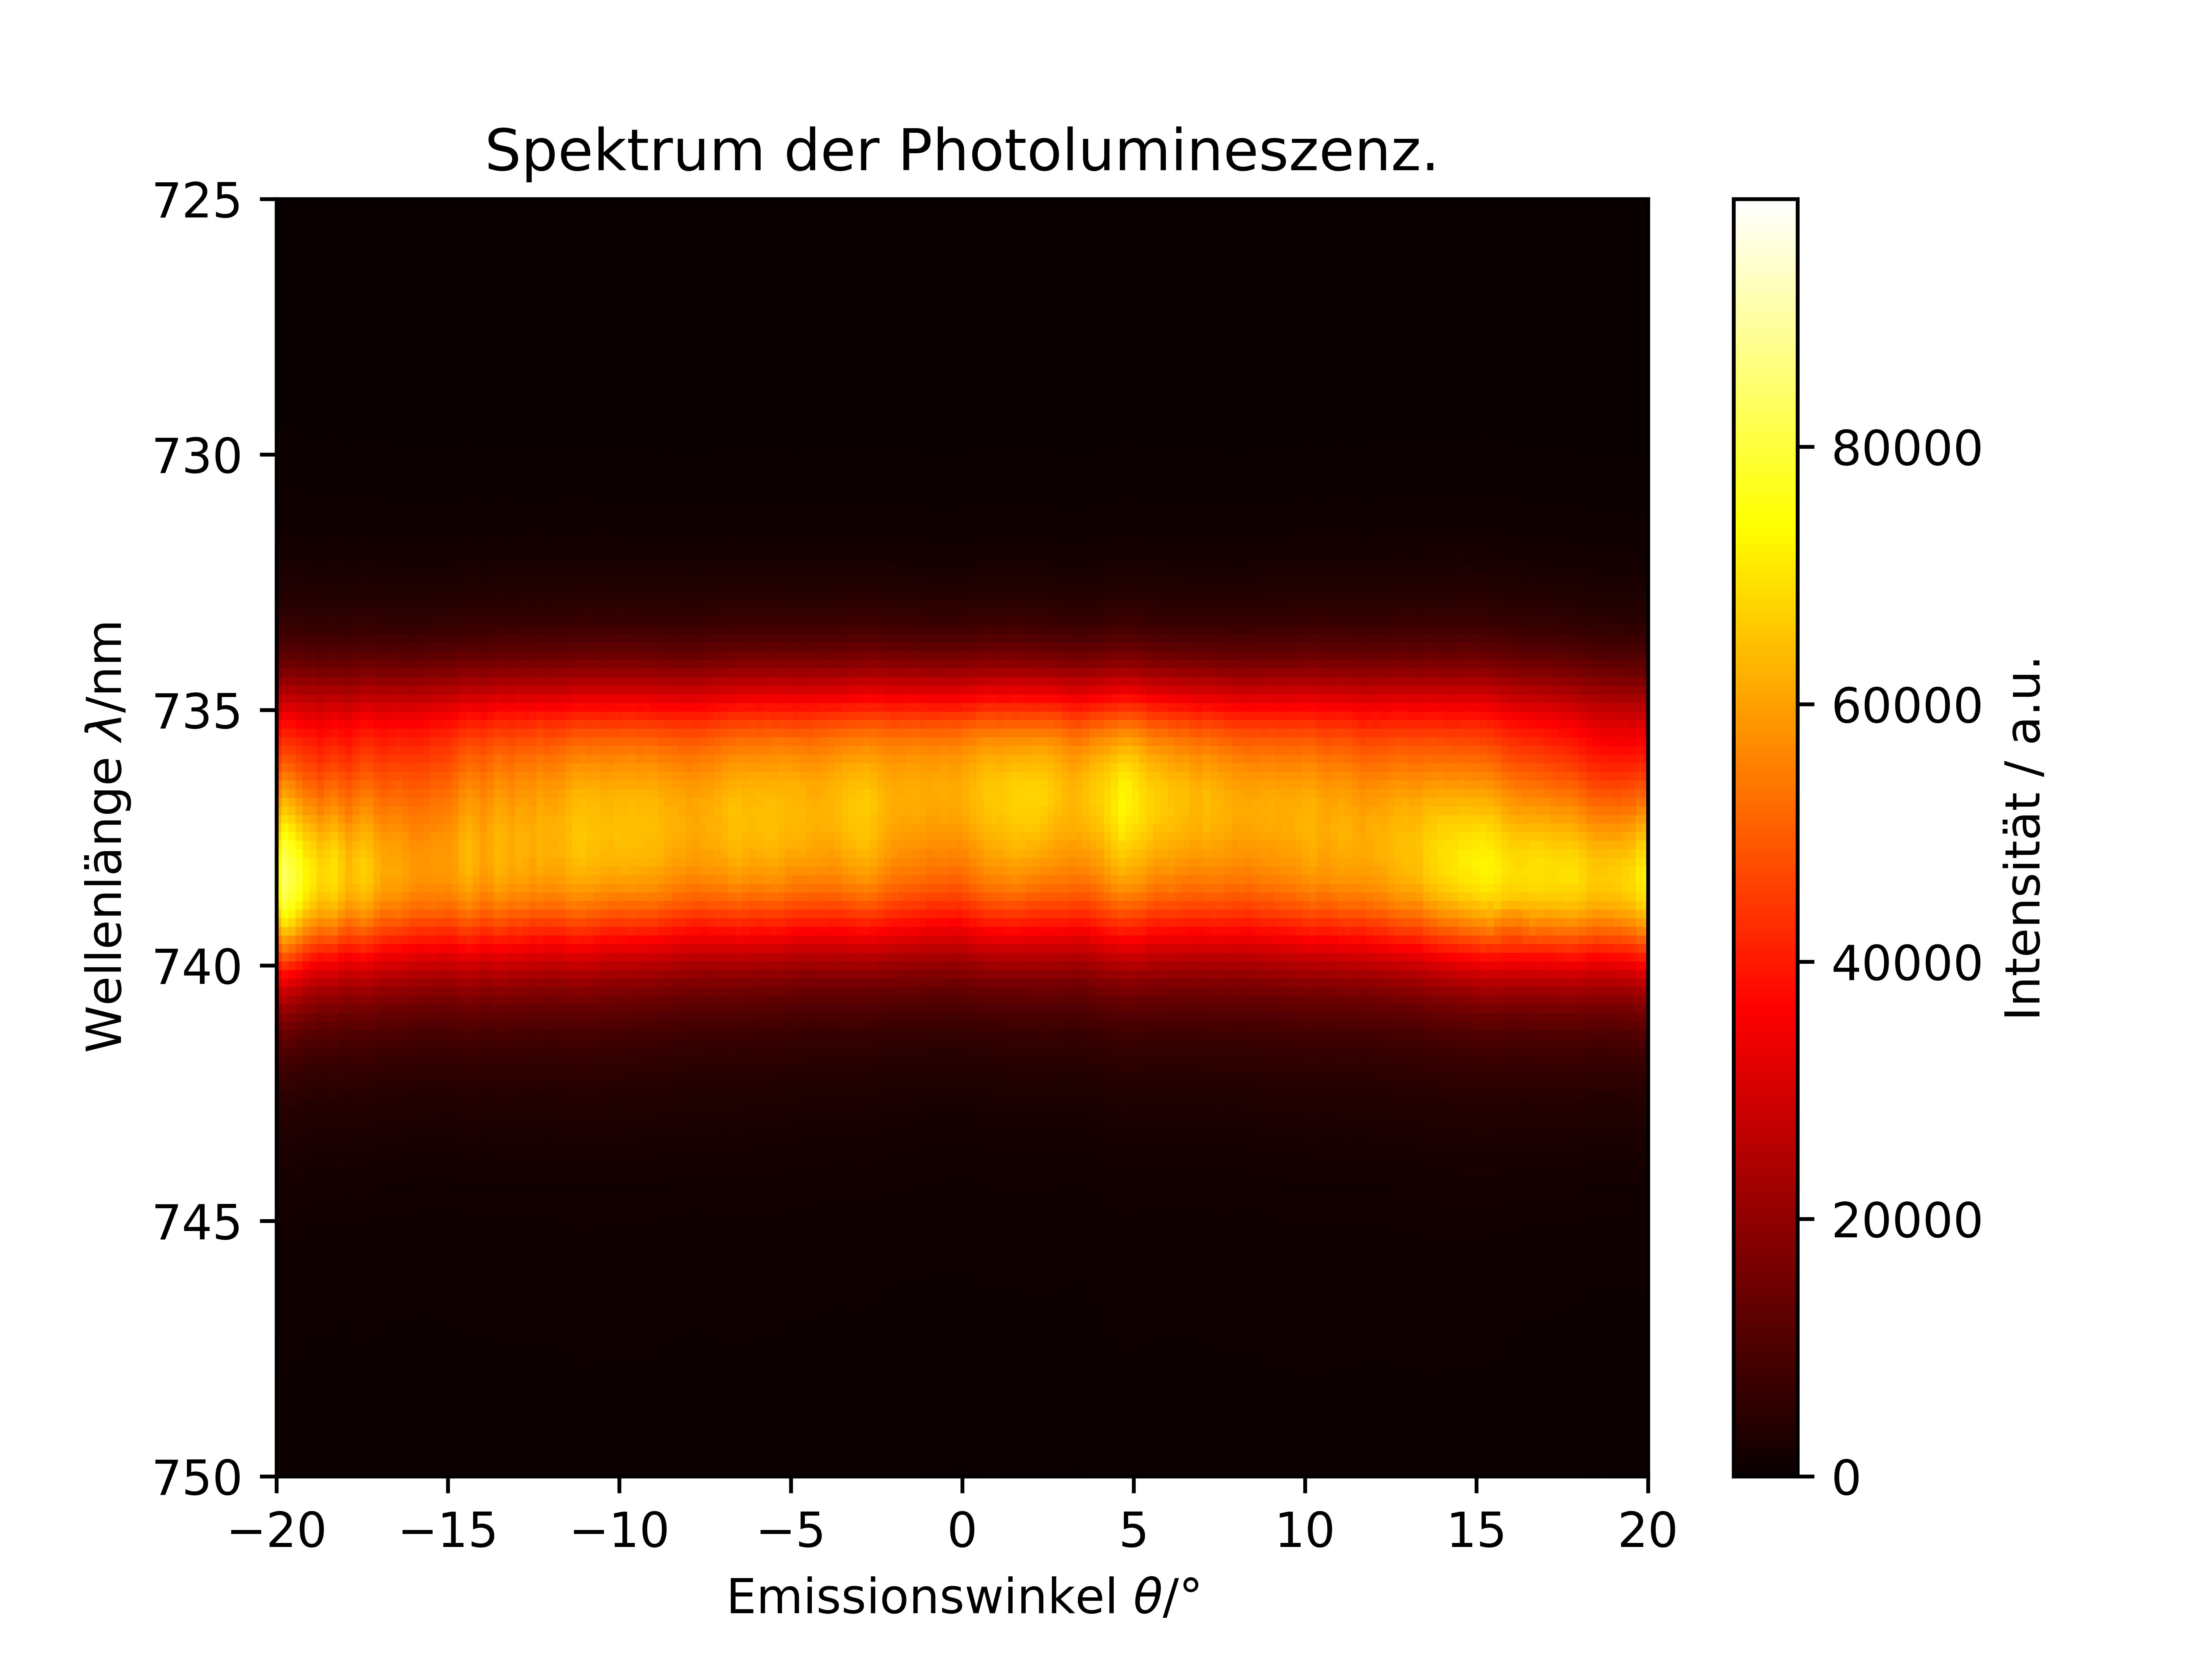
\includegraphics[scale=0.6]{./Plots/colormap__intensity_photolumineszenz_022818A 250nm 4K 2020-07-14.png}
    \caption{Gemessene PL bei einer Temperatur von $\SI{4}{\kelvin}$. 
    Das Maximus ist bei $\SI{738}{\nano\meter}$. 
    Je heller die Bereiche desto mehr Intensität ist an der Stelle gemessen worden.}
    \label{fig:photo}
\end{figure}
\FloatBarrier
%%%%%%%%%%%%%%%%%%%%%%%%%%%%%%%%%%%%%%%%%%%%%%%%%%%%%%%%%%%%%%%%%%%%%%%%%%%%%%%%%%%%%%%%%%%%%%%%%%%
\begin{figure}
    %\centering
    \begin{subfigure}{0.5\textwidth}
        \centering
        \includegraphics[scale=0.45]{./Plots/max_value_Pl.pdf}
        \caption{Darstellung des Intensitätsmaximums, der im Experiment gemessenen Photolumineszenz, der Probe.}
        \label{fig:max}
    \end{subfigure}
    \begin{subfigure}{0.5\textwidth}
        \centering
        \includegraphics[scale=0.45]{./Plots/positive_and_negative_intensity_at_specific_wavelength_738_nm_022818A 250nm 4K 2020-07-14.pdf}
        \caption{Bla bla. scheiß formattier\\
        ung!}
        \label{fig:i_pn}
    \end{subfigure}
    \caption{Unterschrift.}
    \label{fig:rho}
\end{figure}
\FloatBarrier
%%%%%%%%%%%%%%%%%%%%%%%%%%%%%%%%%%%%%%%%%%%%%%%%%%%%%%%%%%%%%%%%%%%%%%%%%%%%%%%%%%%%%%%%%%%%%%%%%%%
%\begin{figure}
%    \centering
%    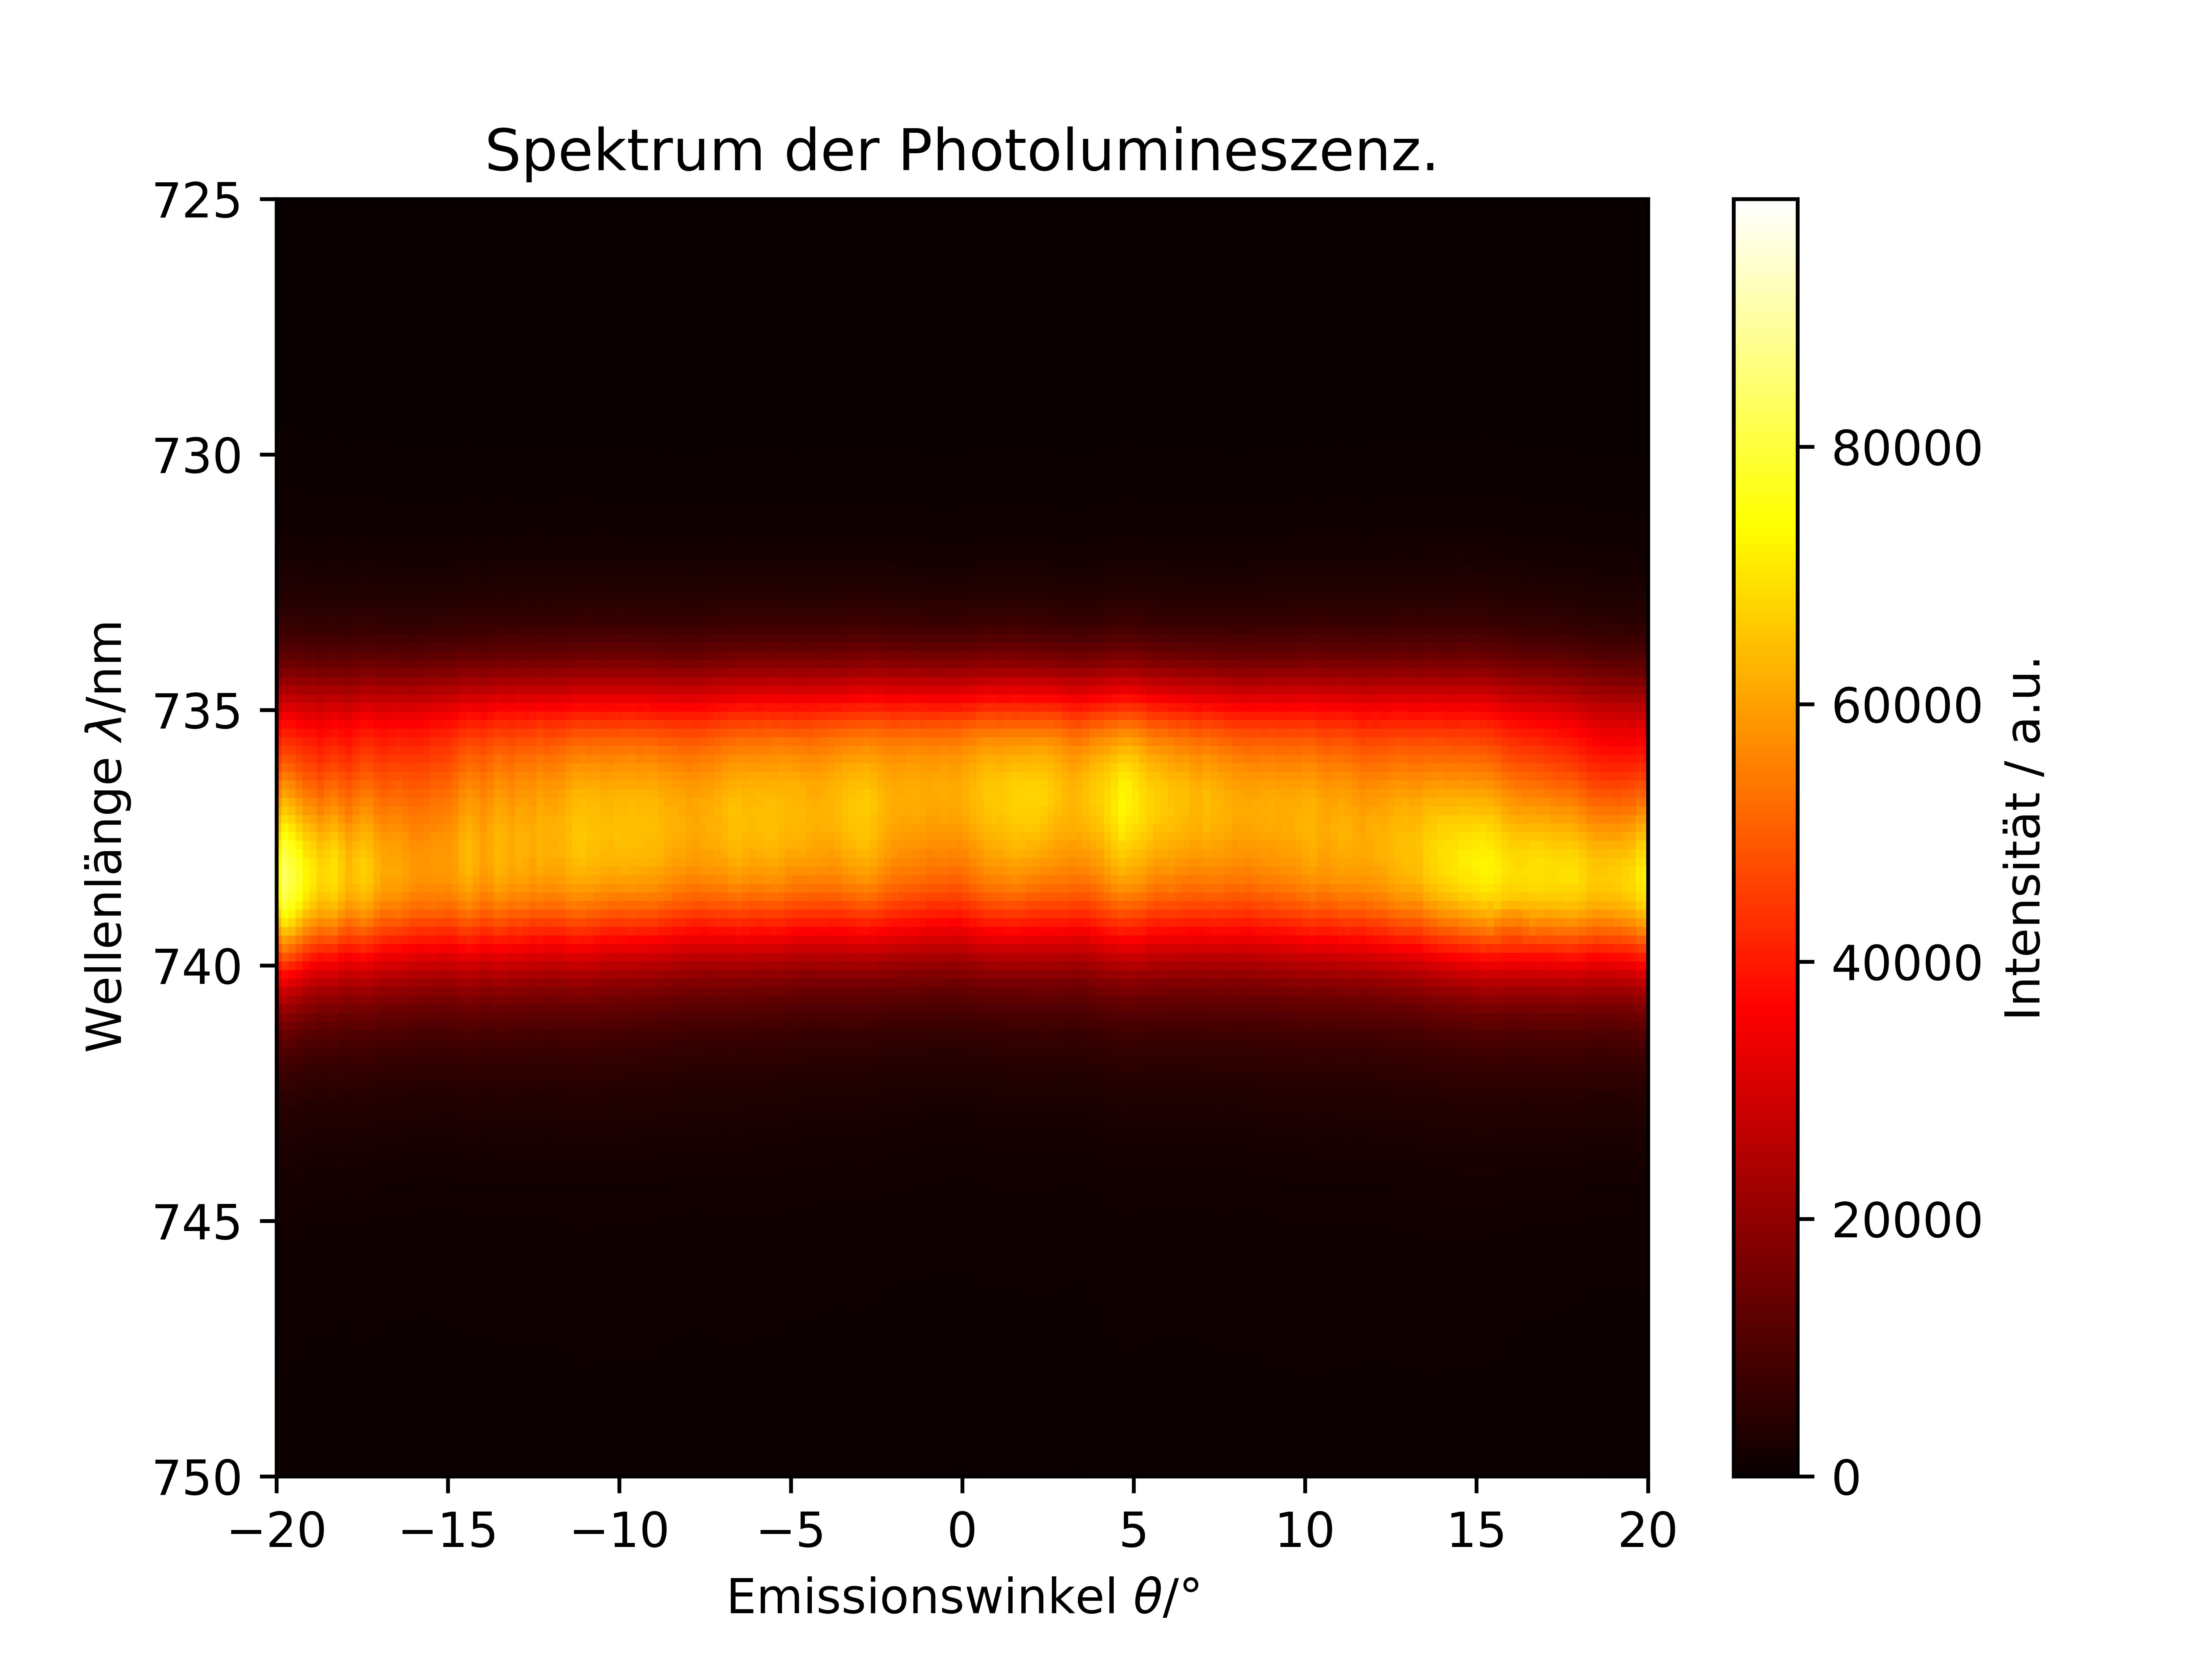
\includegraphics[scale=0.6]{./Plots/colormap__intensity_photolumineszenz_022818A 250nm 4K 2020-07-14.png}
%    \caption{Gemessene PL bei einer Temperatur von $\SI{4}{\kelvin}$. 
%    Das Maximus ist bei $\SI{738}{\nano\meter}$. 
%    Je heller die Bereiche desto mehr Intensität ist an der Stelle gemessen worden.}
%    \label{fig:photo}
%\end{figure}
%\FloatBarrier

Die von der Probe emittierte Wellenlänge liegt im sichtbaren Bereich und war real im Experiment als rotes Licht zu erkennen.
Der Winkelbereich wird bei Winkelabhängigen Messungen auf $\theta = \pm \SI{20}{\degree}$ 
eingeschränkt um störende Randeffekte/Artefakte zu vermeiden. 
Der Tatsächlich auflösbare Winkelbereich, aufgrund der numerischen Apertur, liegt bei $\theta = \pm \SI{24}{\degree}$ 
(vgl. Abschnitt~\ref{sec:Beschreibung des Versuchsaufbaus}).
Die abgebildete PL ist durch die Summation aller Einzelmessungen 
bei positiven und negativen Magnetfeld entstanden. 
Wie in Abbildung~\ref{fig:photo} zu erkennen, ist die Intensität homogen über den Winkelbereich verteilt.
Daraus lässt sich schließen, dass es bei dem Effekt keine bevorzugte Polung des Magnetfelds
geben kann, da sonst farblich hervorgehobene Intensitätsspitzen existieren müssten. 
Die Abnahme der Intensität unter ca. $\SI{735}{\nano\meter}$ und über ca. 
$\SI{740}{\nano\meter}$ bedeuten, dass die Probe ab diesem Wellenlängen fast bis kein Licht mehr emittiert.
Die farblich dargestelle Intensität hat keine weiter spezifizierte physikalische Einheit, da es nur um Änderungen unter
den Intensitäten geht.

Die von der CCD im Experiment erfasste relative Änderung der Intensität (Direktionalität) $\rho$,
des kompletten Sensors, ist in Abbildung~\ref{fig:rel_komplett} zu sehen.
\begin{figure}
    %\centering
    \begin{subfigure}{0.50\textwidth}
        %\centering
        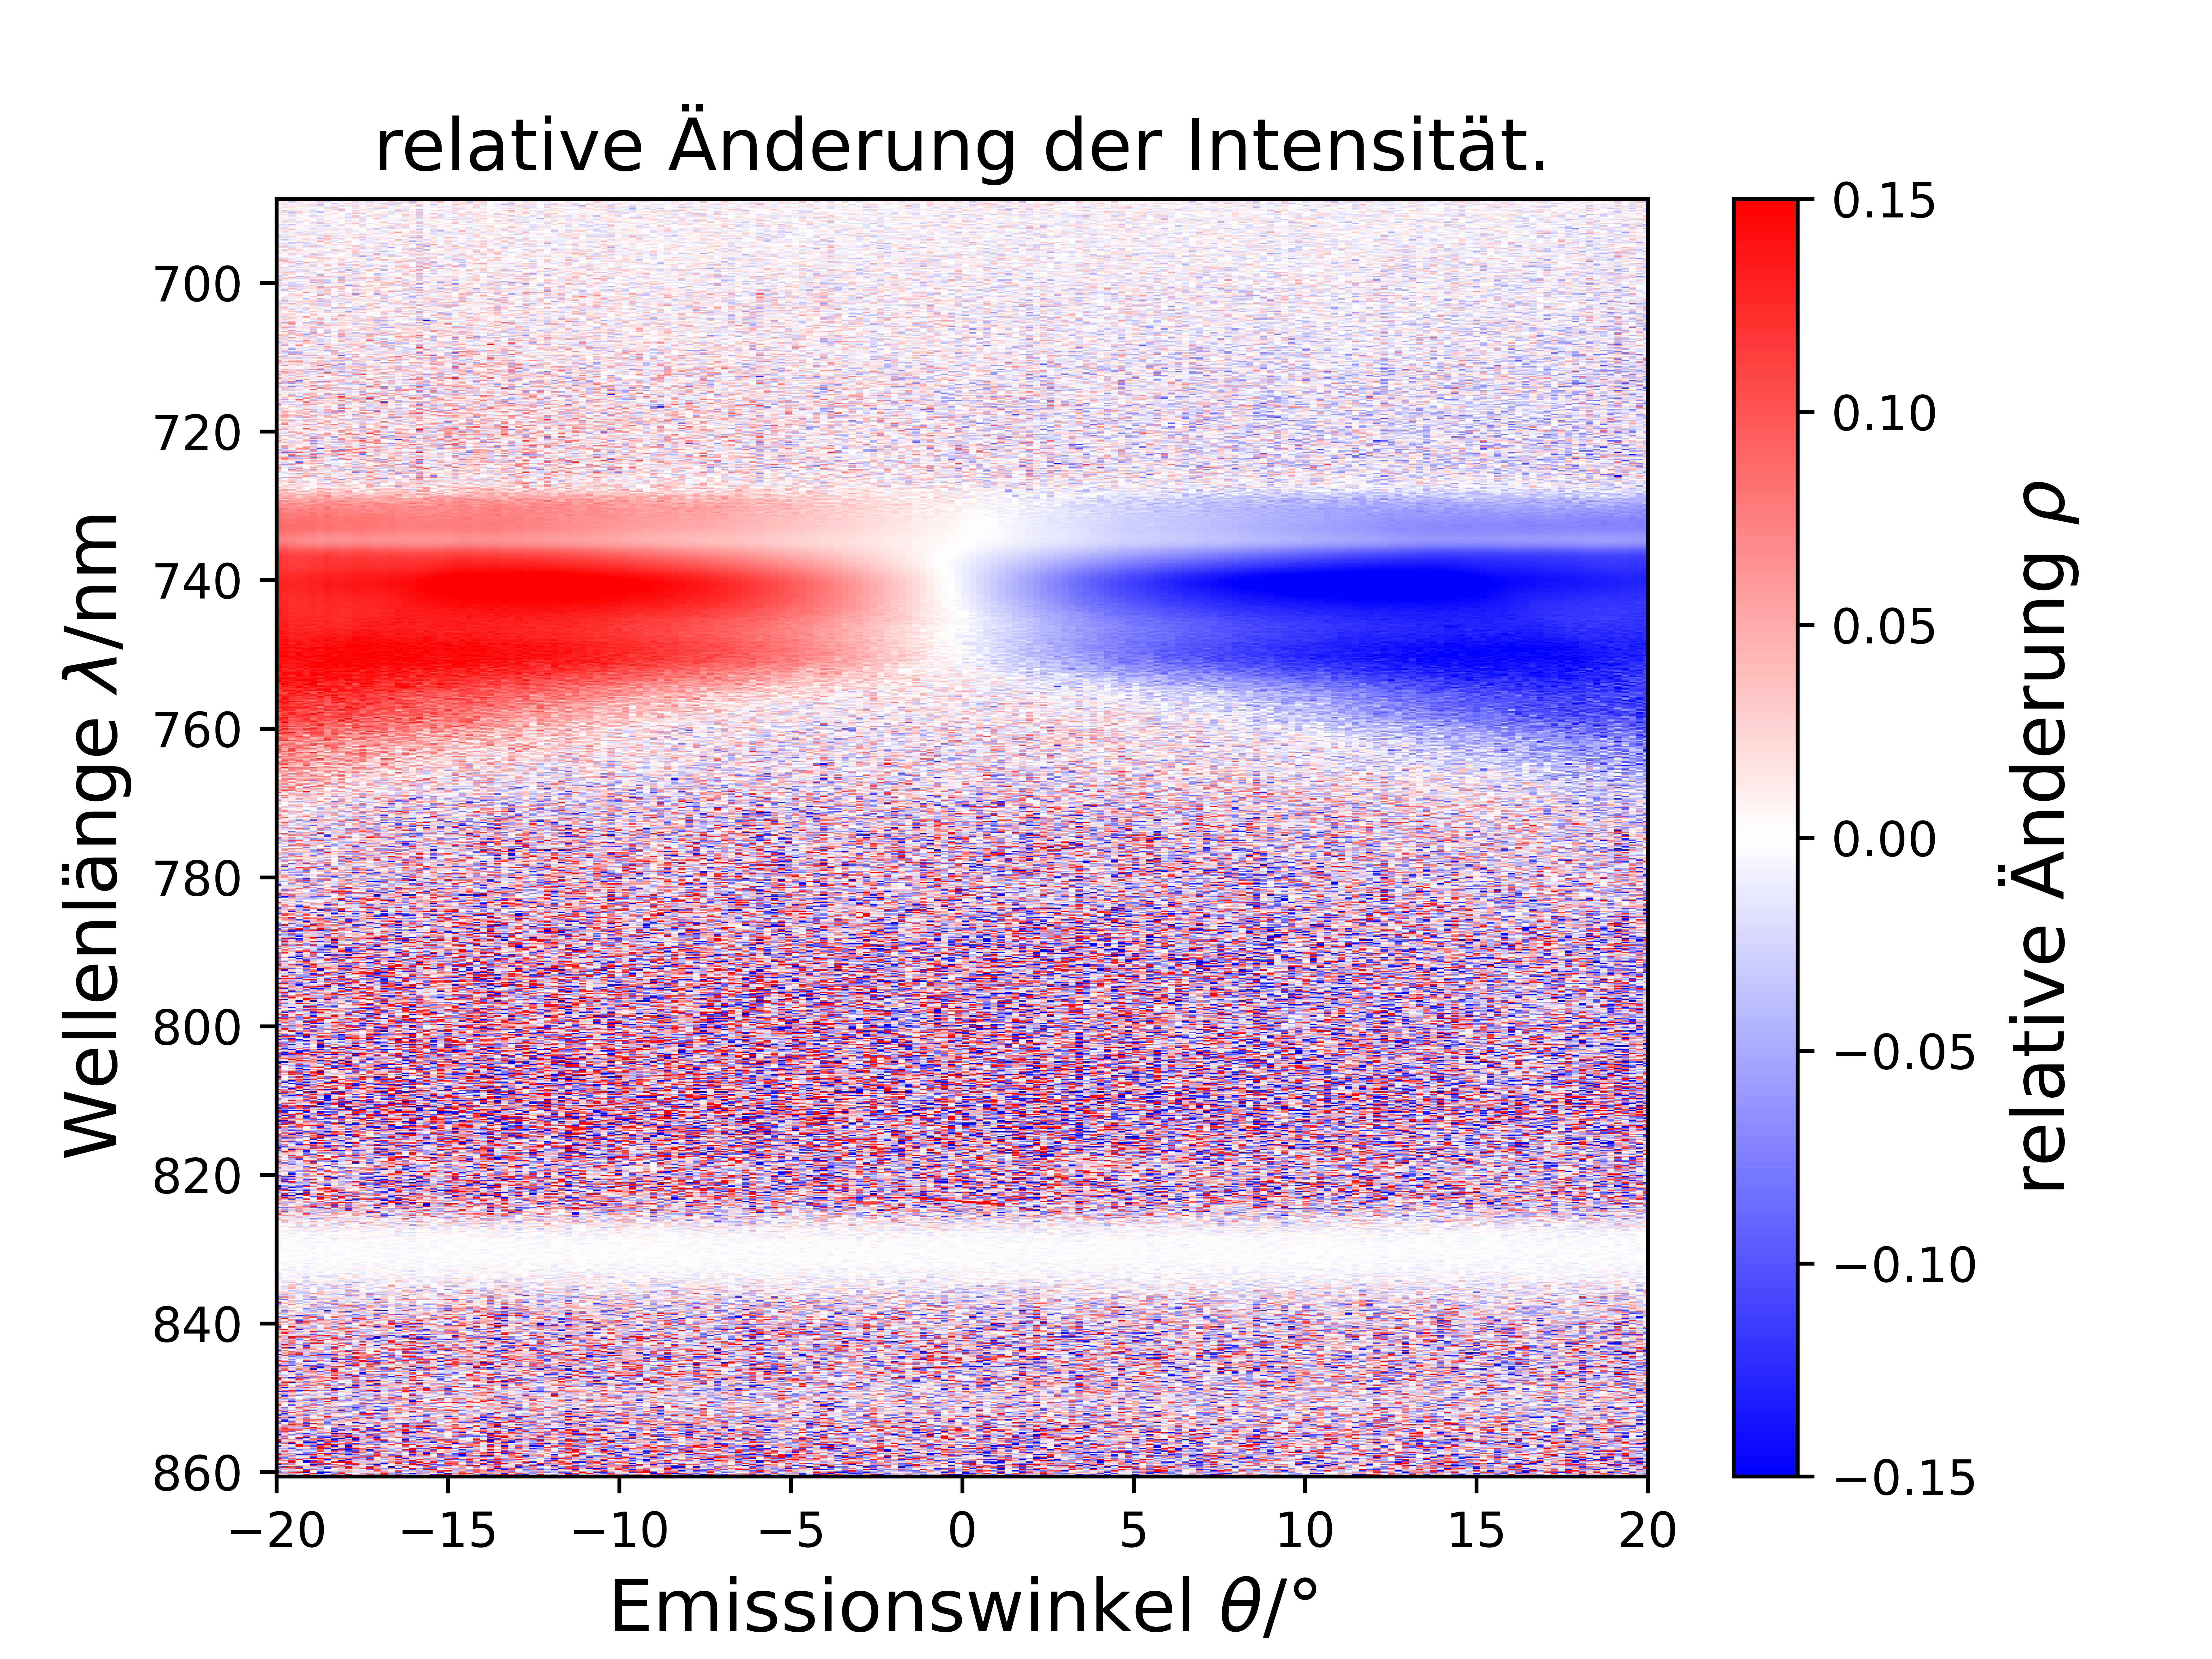
\includegraphics[scale=0.45]{./Plots/colormap_rel_change_intensity_022818A 250nm 4K 2020-07-14_komplett.png}
        \caption{Gemessene Direktionalität, des vollständigen\\ Sensors, bei einer Temperatur von $\SI{4}{\kelvin}$.}
        \label{fig:rel_komplett}
    \end{subfigure}
    \begin{subfigure}{0.50\textwidth}
        %\centering
        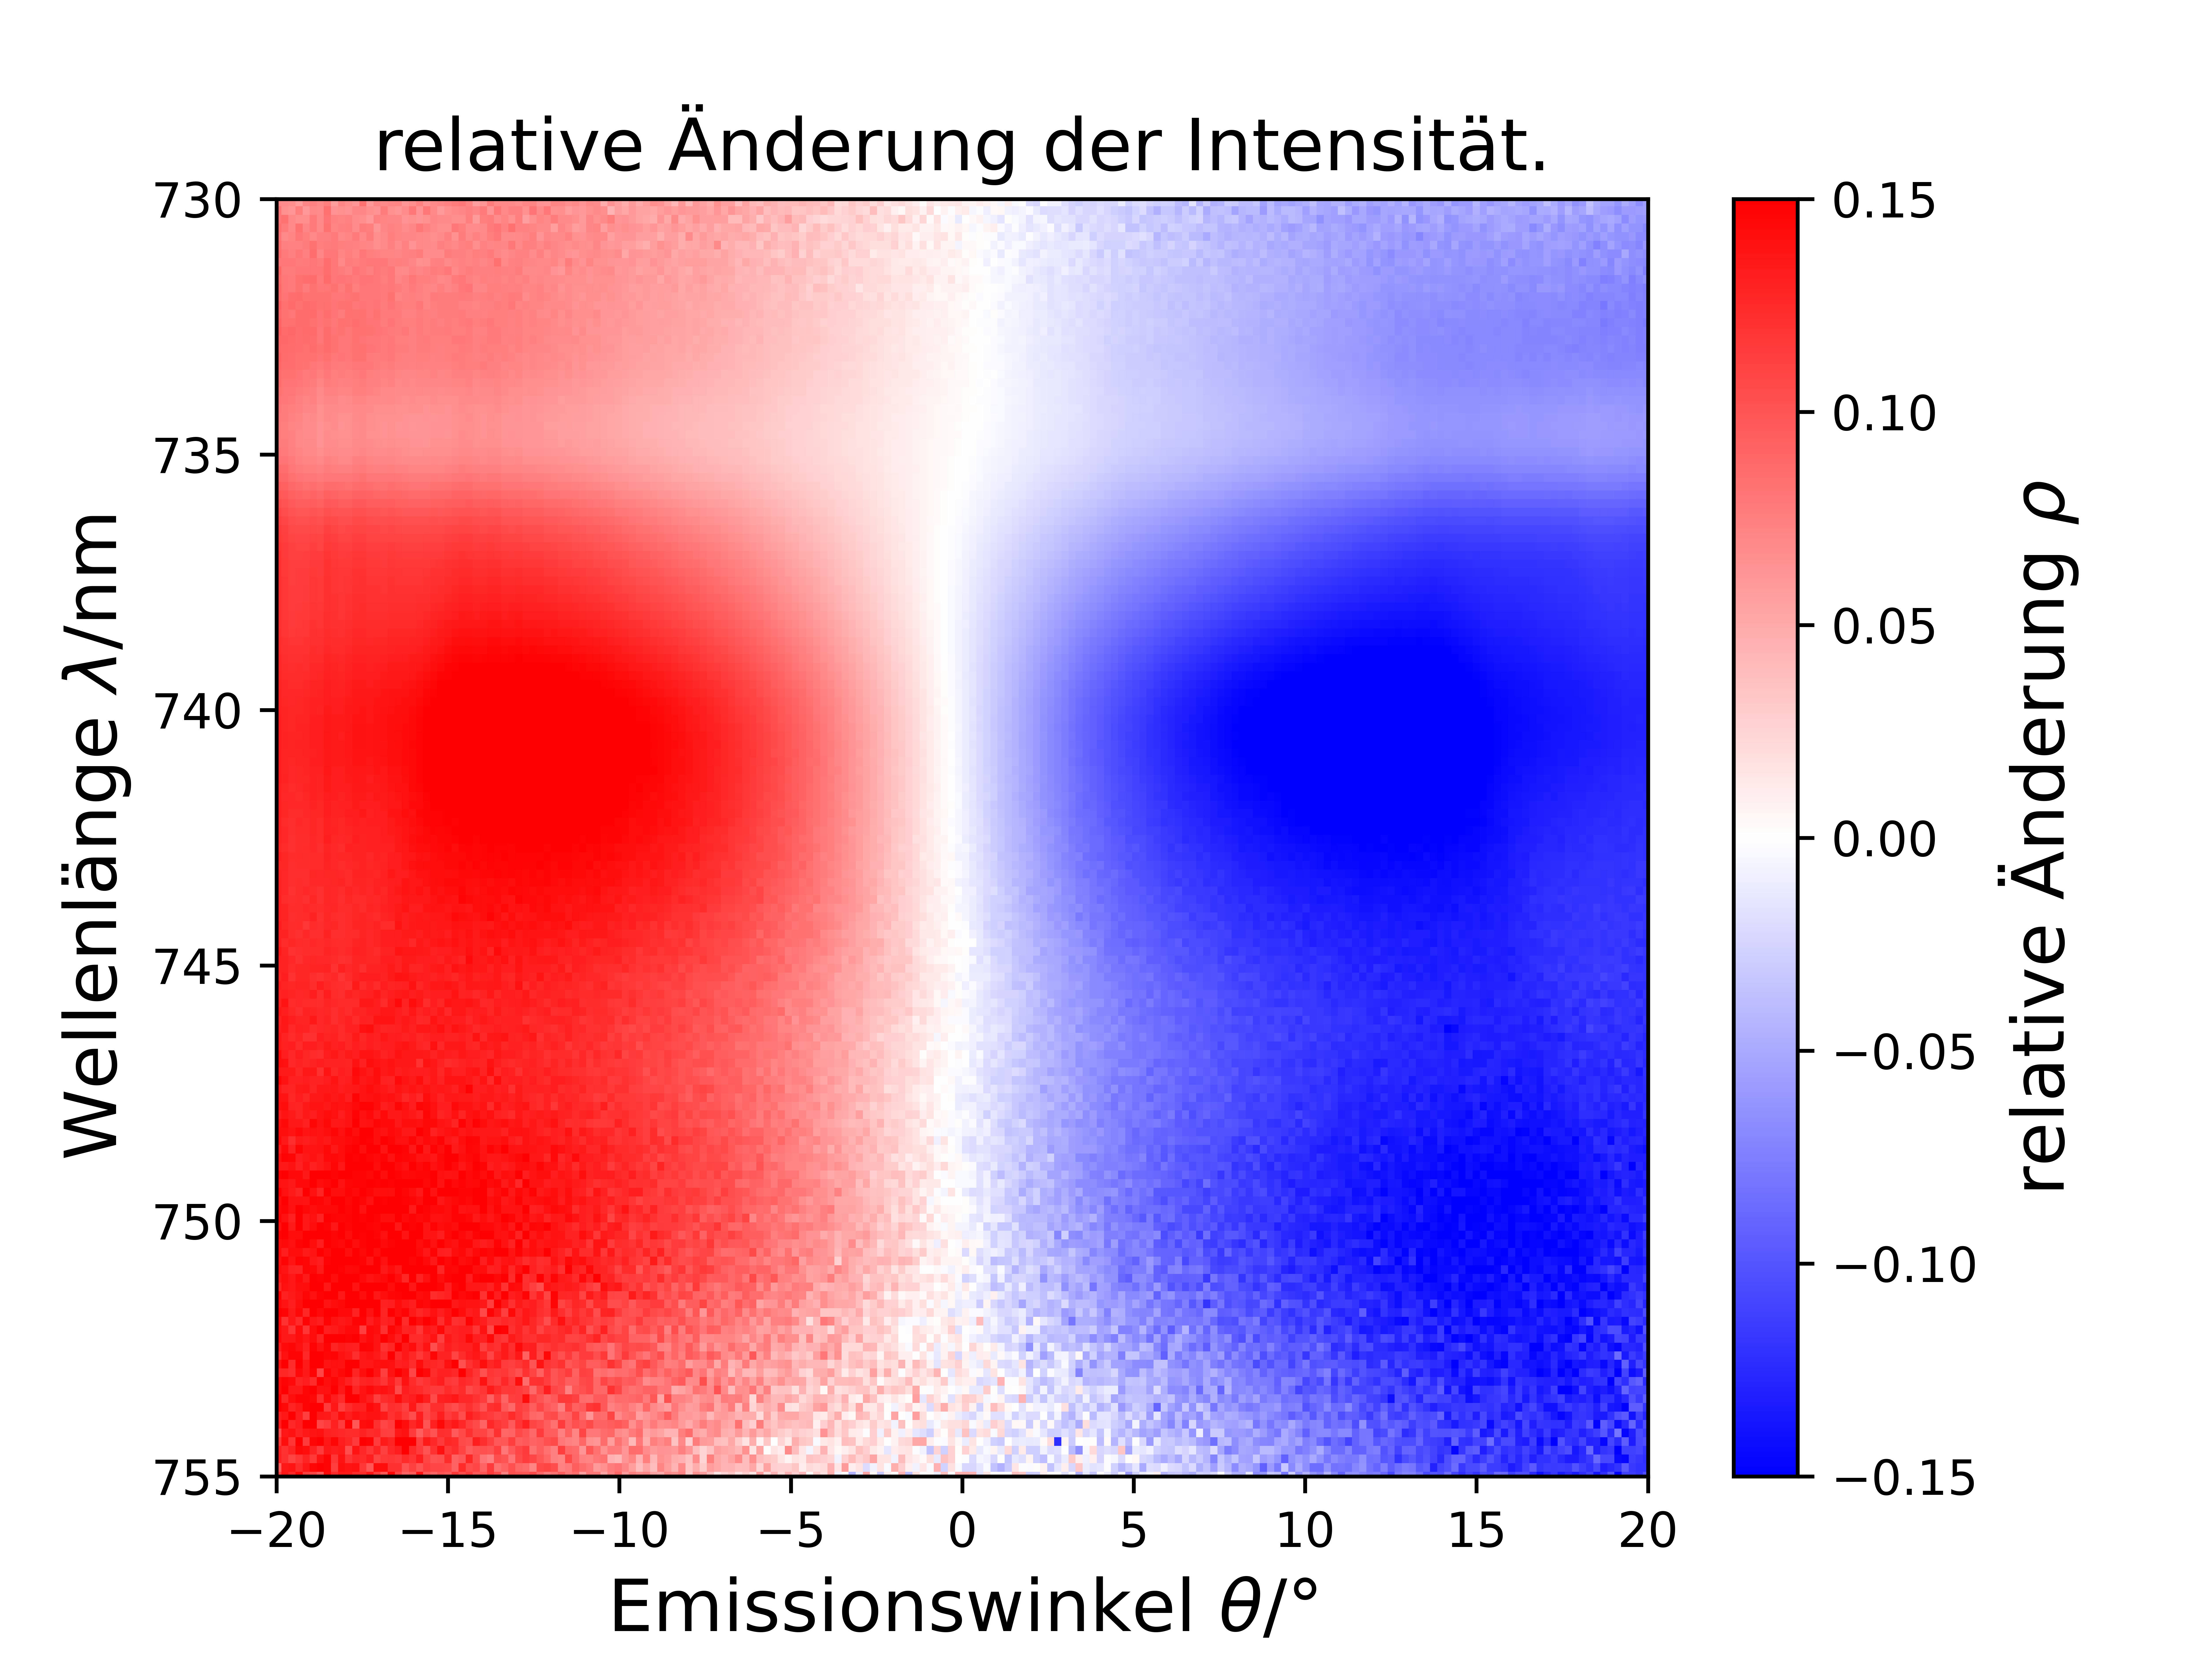
\includegraphics[scale=0.45]{./Plots/colormap_rel_change_intensity_022818A 250nm 4K 2020-07-14.png}
        \caption{Gemessene Direktionalität im Bereich von $\SI{725}{\nano\meter}$ bis $\SI{755}{\nano\meter}$
        bei einer Temperatur von $\SI{4}{\kelvin}$.}
        \label{fig:rel}
    \end{subfigure}
    \caption{Darstellung der Direktionalität in verschiedenen Wellenlängenbereichen.}
    \label{fig:rho}
\end{figure}
\FloatBarrier

Die Direktionalität $\rho$ berechnet sich durch 
\begin{equation}
    \rho = \frac{I_\text{B+} - I_\text{B-} }{ I_\text{B+} + I_\text{B-} }.
\end{equation}
Dabei ist $I_\text{B+}$ die Intensität bei positiven Magnetfeld und $I_\text{B-}$ bei negativen Magnetfeld.
Die Direktionalität in Prozent gibt an, wie sehr sich die Lichtemission in eine Richtung bei Umpolung des Magnetfelds ändert. 
Der Maximalwert von $\rho$ beträgt somit $1$.
Eine farbliche Darstellung ist in Abbildung~\ref{fig:rel_komplett}zu sehen.
Der maximal gemessene Wert der Direktionalität im Experiment beträgt $\pm \SI{15}{\percent}$. 
Das bedeutet konkret, dass das ausgesendete Licht der Probe, die PL, $\SI{15}{\percent}$ stärker in eine Richtung
emittiert wird, wenn das Magnetfeld eine bestimmte Polung besitzt.
Der weisse Balken der im Wellenlängenbereich von ca. $\SI{825}{\nano\meter}$ bis $\SI{835}{\nano\meter}$ 
in Abbildung\ref{fig:rel_komplett} zu sehen ist, 
hat seinen Ursprung im verwendten Substrat GaAs. Da dieses ebenfalls zum Leucheten angeregt wird.
GaAs hat allerdings keine magnetischen Eigenschaften, darum entfällt die Beeinflussung durch das angelegte Magnetfeld
und es ist keine Direktionalität erkennbar.
 % GaAs strahlt aber wie und warum ? da es nicht magnetisch ist 
%kann ist es unempfunlich gegeb das magnetfelg ==> kein effekt
Der Restbereich, d.h. der Bereich ohne Signifikanten Effekt, besteht aus einem statistischen Pixelrauschen der CCD.

In Abbildung~\ref{fig:rel} ist der reine Bereich der Direktionalität dargestellt.
Hier ist ebenfalls eine weisse Linie (vertikal) in der Mitte des Graphen bei $\theta = \SI{0}{\degree}$ zu erkennen.
Dieser Bereich entsteht da bei einem Winkel von $\theta = \SI{0}{\degree}$ das PL genau senkrecht aus der Probe kommt
und somit keine Direktionalität aufweisen kann.
Die schwächere horizontale Linie bei $\lambda = \SI{735}{\nano\meter}$ 
(vgl. Abbildung~\ref{fig:rho}) entsteht durch 
ausgesendetes Licht der Probe welches sich mit dem eigentlichen Effekt überlagert. 
Es wird vermutet das dieses Licht aus den Randbereichen der Probe und/oder aus den Zwischenbereichen des Goldgitters 
emittiert wird.

Die Direktionalität im Maximum der Photolumineszenz (bei $\lambda = \SI{738}{\nano\meter}$) beträgt
$\rho = \SI{13}{\percent}$. 
Dieser Verlauf der Direktionalität bei konstanter Wellenlänge ist in Abbildung~\ref{fig:dir} dargestellt.
\begin{figure}
    \centering
    \includegraphics[scale=0.6]{./Plots/rho_at_specific_wavelength_738_nm_022818A 250nm 4K 2020-07-14.pdf}
    \caption{Gemessene Direktionalität $\rho$ im Maximum der Photolumineszenz.
    Der Wert der im Experiment gemessen Direktionalität ist $\rho = \SI{13}{\percent}$.}
    \label{fig:dir}
\end{figure}
\FloatBarrier

Der Graph von $\rho$ ist bis auf eine kleine Abweichung am Nullpunkt (vgl. Abbildung~\ref{fig:dir}) 
Spiegelsymmetrisch. 
Das Ergebnis der Spiegelsymmetrie ist mit der Theorie im Einklang, denn das einzige was eine
Änderung des Magnetfelds bewirkt ist ein Vorzeichenwechsel der Direktionalität.
Bis ca. $\theta = \pm \SI{5}{\degree}$ ist die Steigung von $\rho$ linear.
Ab diesem Wert geht der Graph in eine Krümmung über die bei $\theta = \pm \SI{13,5}{\degree}$
ihr Maximum besitzt. 
Hinter dem Maximum schwächt sich die Direktionalität ab.

Der Graph von $\rho$ lässt sich mit der Gleichung 
\begin{equation}
    c_0= \frac{\rho(-\theta)-\rho(\theta)}{2}
    \label{eq:c_0} 
\end{equation}

um den Nullpunkt korrigieren, sodass er perfekt achsensymmetrisch ist.
Dies ist in Abbildung~\ref{fig:dir_kor} zu sehen.
\begin{figure}
    \centering
    \includegraphics[scale=0.6]{./Plots/rho_at_specific_wavelength_738_nm_022818A 250nm 4K 2020-07-14_korrigiert.pdf}
    \caption{Gemessene um den Nullpunkt korrigierte Direktionalität $c_0$ im Maximum der Photolumineszenz.
    Der Wert der im Experiment gemessen Direktionalität ist $\rho = \SI{13}{\percent}$.}
    \label{fig:dir_kor}
\end{figure}
\FloatBarrier


bla bla bla